\documentclass[20pt, a0paper, portrait]{tikzposter} % Уменьшен шрифт до 20pt

\usepackage[utf8]{inputenc} 
\usepackage[russian, english]{babel}
\usepackage{amsmath, amsfonts, amssymb}
\usepackage{booktabs, array, xcolor, graphicx}
\usepackage{enumitem}

% Настройка полей, чтобы текст не прижимался к краям
\geometry{paperwidth=841mm, paperheight=1189mm, margin=2cm}

\definecolor{DarkTeal}{HTML}{173A4A} 
\definecolor{LightTeal}{HTML}{D5E6EA}
\definecolor{BlockGray}{HTML}{F4F6F7} 
\definecolor{Highlight}{HTML}{2D7A77}

\usetheme{Default} 
\colorlet{backgroundcolor}{LightTeal}
\colorlet{titlebgcolor}{DarkTeal} 
\colorlet{titlefgcolor}{white}
\colorlet{blocktitlebgcolor}{DarkTeal} 
\colorlet{blocktitlefgcolor}{white}
\colorlet{blockbodybgcolor}{BlockGray}

\title{\parbox{\linewidth}{\centering
Evaluating Relation Extraction Strategies\\
for Knowledge Graph Construction}} 
\author{Dmitriy Ryazanov \quad \texttt{d.ryazanov@innopolis.university}} 
\institute{Innopolis University \quad | \quad Natural Language Processing Track}

\begin{document} 
\maketitle

\begin{columns} 
\column{0.5} % ЛЕВАЯ КОЛОНКА

\block{Motivation}{ 
    \textbf{Goal:} identify the most reliable relation extraction setup for downstream KG writing.
    \vspace{0.4cm}
    \begin{itemize}[leftmargin=*, noitemsep]
        \item Compare heuristic, classical, and neural RE approaches.
        \item Measure quality under different entity encoding strategies.
        \item Derive a practical policy for safe KG insertion.
    \end{itemize}
}

\block{Experimental Setup}{
    \begin{minipage}{0.48\linewidth}
        \textbf{Data Tracks:}
        \begin{itemize}[leftmargin=*, noitemsep]
            \item Synthetic (Hard/Adv/Noisy)
            \item SemEval-2010 Task 8
            \item AG News, DBPedia, Yelp
        \end{itemize}
    \end{minipage}
    \hfill
    \begin{minipage}{0.48\linewidth}
        \textbf{Models:}
        \begin{itemize}[leftmargin=*, noitemsep]
            \item Dependency Rules, OpenIE
            \item TF-IDF + (SVM/LR/RF)
            \item SentenceTransformer
        \end{itemize}
    \end{minipage}
}

\block{Methods}{
    \small
    \textbf{RE pipeline:}
    \begin{enumerate}[leftmargin=*, noitemsep]
        \item Parse sentence + entity pair $(e_1,e_2)$.
        \item Build text variant: \texttt{raw} / \texttt{masking} / \texttt{markers}.
        \item Train or apply extractor (Rules, OpenIE, TF-IDF classifier, SBERT head).
        \item Predict relation label and confidence score.
    \end{enumerate}

    \vspace{0.2cm}
    \textbf{Compared model families:}
    \begin{itemize}[leftmargin=*, noitemsep]
        \item \textbf{Dependency Rules:} high precision, template-sensitive recall.
        \item \textbf{OpenIE-style:} triple extraction + mapping to target relation set.
        \item \textbf{Classical ML:} TF-IDF + SVM/LR/NB/RF.
        \item \textbf{Neural:} SentenceTransformer embeddings + PyTorch classification head.
    \end{itemize}

    \vspace{0.2cm}
    \textbf{Evaluation protocol:}
    \begin{itemize}[leftmargin=*, noitemsep]
        \item Main quality: Macro-F1 and MCC (class imbalance aware).
        \item Ranking quality: PR-AUC and ROC-AUC.
        \item Efficiency: runtime and neural/classical runtime ratio.
        \item Error profile: boundary errors and relation-label confusion.
    \end{itemize}

    \vspace{0.2cm}
    \textbf{KG decision rule:}
    \begin{itemize}[leftmargin=*, noitemsep]
        \item Per-relation confidence thresholds (\texttt{accept}/\texttt{review}).
        \item Queue-based output: \texttt{accept}, \texttt{review}, \texttt{reject}.
    \end{itemize}
}

\block{Experimental Results}{ 
    \small 
    \textbf{SemEval strict protocol (Top-5, mean results):} \\
    \begin{center}
    \begin{tabular}{l c c}
        \toprule 
        \textbf{Config} & \textbf{Macro-F1} & \textbf{MCC} \\ 
        \midrule 
        \textbf{SVM + markers} & \textbf{0.736} & \textbf{0.679} \\ 
        NB + markers & 0.720 & 0.676 \\ 
        LogReg + markers & 0.718 & 0.655 \\ 
        SVM + raw & 0.692 & 0.629 \\
        RF + markers & 0.684 & 0.608 \\
        \bottomrule 
    \end{tabular}
    \end{center}
    
    \vspace{0.3cm}
    \textbf{Representation Performance (Aggregated):}
    \begin{itemize}[leftmargin=*]
        \item \textbf{Markers (0.714)} $>$ Raw (0.684) $>$ Masking (0.661)
        \item SVM + markers peaked at \textbf{0.747} F1.
    \end{itemize}

    \vspace{0.2cm}
    \textbf{Heuristic vs Supervised on Synthetic-Hard:}
    \begin{itemize}[leftmargin=*, noitemsep]
        \item TF-IDF+LR and SBERT reached \textbf{1.000} Macro-F1.
        \item OpenIE: \textbf{0.747} Macro-F1 (boundary errors observed).
        \item Dependency Rules: \textbf{0.716} Macro-F1.
    \end{itemize} 

    \vspace{0.25cm}
    \textbf{External datasets (Best model per dataset):}\\[-0.1cm]
    \begin{center}
    \begin{tabular}{l l c}
        \toprule
        \textbf{Dataset} & \textbf{Winner} & \textbf{Macro-F1} \\
        \midrule
        ag\_news & SBERT + TorchHead & 0.849 \\
        dbpedia\_14 & SBERT + TorchHead & 0.946 \\
        yelp\_polarity & TF-IDF + LR & 0.825 \\
        sem\_eval\_2010\_task\_8 & TF-IDF + LR & 0.630 \\
        \bottomrule
    \end{tabular}
    \end{center}

    \vspace{0.2cm}
    \textbf{Neural vs Classical trade-off (delta F1 / runtime ratio):}
    \begin{itemize}[leftmargin=*, noitemsep] 
        \item \textbf{AG News:} $+0.076$ / $\times 150.6$ (quality gain, very expensive).
        \item \textbf{DBPedia:} $+0.019$ / $\times 27.6$ (small gain).
        \item \textbf{Yelp:} $-0.025$ / $\times 126.3$ (classical preferred).
        \item \textbf{SemEval subset:} $-0.256$ / $\times 41.2$ (classical clearly better).
    \end{itemize}

    \vspace{0.2cm}
    \textbf{Stress tests:}
    \begin{itemize}[leftmargin=*, noitemsep]
        \item Synthetic-Imbalanced: LR 1.000 vs SBERT 0.995 Macro-F1.
        \item Synthetic-Noisy: LR 0.897 vs SBERT 0.887 Macro-F1.
        \item Noise affected performance more than class imbalance.
    \end{itemize}

    \vspace{0.2cm}
    \textbf{Error profile highlights:}
    \begin{itemize}[leftmargin=*, noitemsep]
        \item Best SemEval model (SVM + markers): label-confusion share \textbf{0.245}.
        \item OpenIE baseline: boundary error rate \textbf{0.081} on Synthetic-Hard.
        \item Dominant practical risk for KG is relation confusion, not extraction failure.
    \end{itemize}
}

\block{KG Output Policy}{ 
    \small
    \textbf{Deployment Model:} \texttt{TF-IDF + LogReg}.\\
    \textit{Rationale:} on SemEval subset, neural variant underperformed ($-0.256$ Macro-F1) and was $\times 41.2$ slower.
    
    \vspace{0.35cm}
    \textbf{Thresholds \& Queue Strategy:}
    \begin{center}
    \begin{tabular}{l c c}
        \toprule
        Relation Type & Accept & Review \\
        \midrule
        Entity-Destination & 0.84 & 0.71 \\
        Cause-Effect & 0.83 & 0.70 \\
        Component-Whole & 0.56 & 0.48 \\
        Product-Producer & 0.51 & 0.43 \\
        \bottomrule
    \end{tabular}
    \end{center}
    
    \vspace{0.2cm}
    \textbf{Decision rule:}
    \begin{itemize}[leftmargin=*, noitemsep]
        \item Write to KG if $p(r|x)\ge \tau_{\texttt{accept}}(r)$.
        \item Send to review if $\tau_{\texttt{review}}(r)\le p(r|x)<\tau_{\texttt{accept}}(r)$.
    \end{itemize}

    \vspace{0.1cm}
    \textbf{Queue outcomes (total 619 triples):}
    \begin{itemize}[leftmargin=*, noitemsep]
        \item Accept: \textbf{156} (\textbf{25.2\%})
        \item Review: \textbf{103} (\textbf{16.6\%})
        \item Reject: \textbf{360} (\textbf{58.2\%})
    \end{itemize}

    \vspace{0.15cm}
    \textbf{Queue examples:}
    \begin{center}
    \begin{tabular}{l l c c}
        \toprule
        e1 & relation & e2 & conf. \\
        \midrule
        metacorpora & Entity-Destination & isthmus & 0.993 \\
        plight & Entity-Destination & dwellers & 0.843 \\
        \bottomrule
    \end{tabular}
    \end{center}
}

\column{0.5} % ПРАВАЯ КОЛОНКА

\block{Visual Dashboard}{ 
    \begin{tikzfigure}[Best SemEval model (SVM + markers): class profile + PR]
        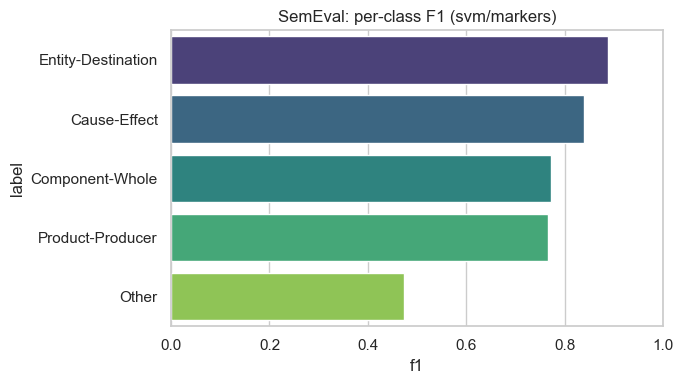
\includegraphics[width=0.48\linewidth, height=9cm, keepaspectratio]{caseStudy_v2_export/images/cell_040_out_07.png}
        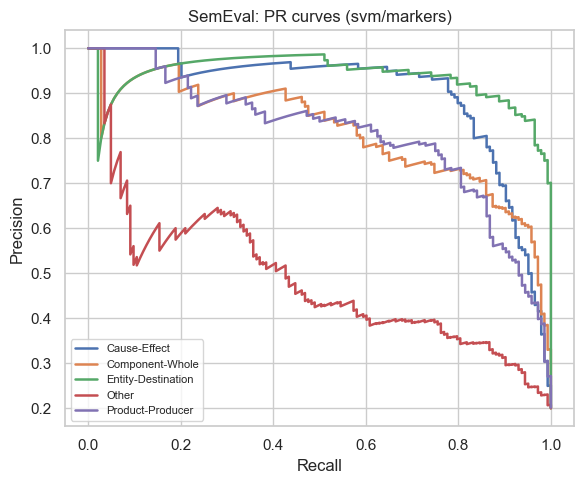
\includegraphics[width=0.48\linewidth, height=9cm, keepaspectratio]{caseStudy_v2_export/images/cell_040_out_08.png}
    \end{tikzfigure}

    \vspace{0.5cm}
    \begin{tikzfigure}[SemEval Mode Heatmap (Cell 50)]
        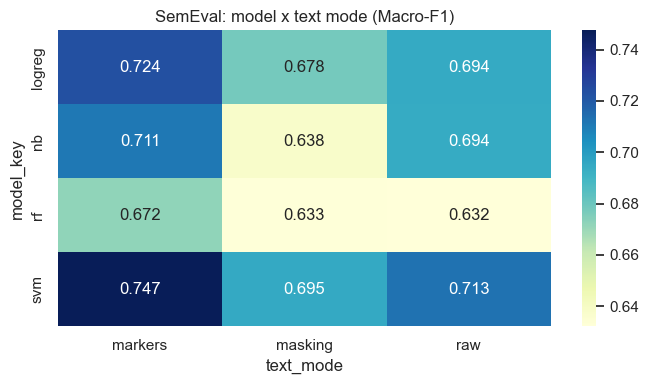
\includegraphics[width=0.9\linewidth, height=14cm, keepaspectratio]{caseStudy_v2_export/images/cell_050_out_02.png}
    \end{tikzfigure}

    \vspace{0.5cm}
    \begin{tikzfigure}[SemEval strict protocol: top configurations]
        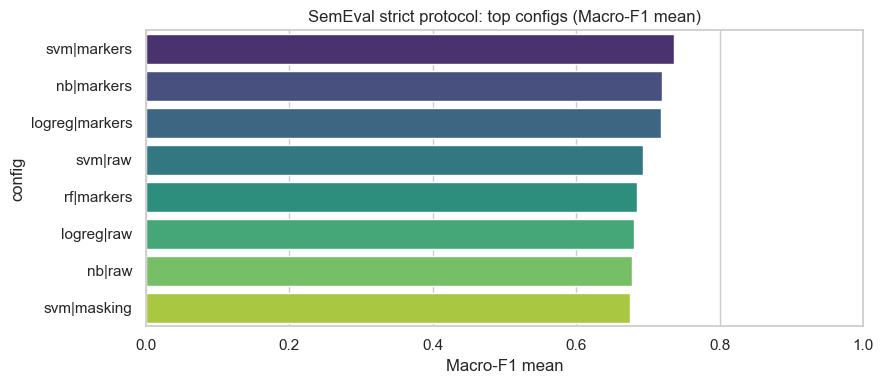
\includegraphics[width=0.9\linewidth, height=10cm, keepaspectratio]{caseStudy_v2_export/images/cell_050_out_04.png}
    \end{tikzfigure} 
    
    \vspace{0.5cm}
    \begin{tikzfigure}[Final KG Construction (Cell 54)]
        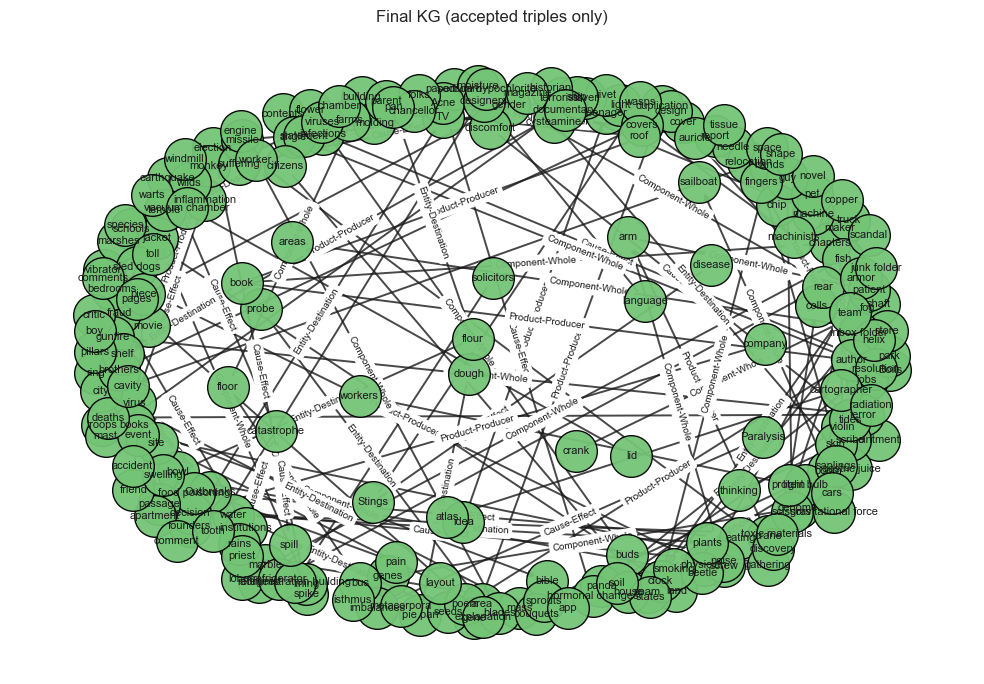
\includegraphics[width=0.9\linewidth, height=14cm, keepaspectratio]{caseStudy_v2_export/images/cell_054_out_06.png}
    \end{tikzfigure}
}

\block{Conclusions}{ 
    \normalsize
    \begin{itemize}[leftmargin=*, itemsep=8pt, label=\textcolor{Highlight}{$\blacksquare$}] 
        \item \textbf{Primary empirical result:} for SemEval-style relation extraction, entity markers provide the most stable quality profile. The best classical configuration (\textbf{SVM + markers}) achieves Macro-F1 \textbf{0.736} (mean protocol) and reaches \textbf{0.747} in the top leaderboard run.
        \item \textbf{Model family conclusion:} classical pipelines (SVM/LR with TF-IDF) remain the strongest default for production throughput, while neural models are beneficial only in selective cases (e.g., AG News), and can be prohibitively expensive in runtime.
        \item \textbf{Cost-quality trade-off:} external evaluation shows that neural gains are dataset-dependent: from a meaningful gain on AG News ($+0.076$ Macro-F1) to underperformance on SemEval subset ($-0.256$), often with large latency multipliers.
        \item \textbf{KG deployment recommendation:} use \texttt{TF-IDF + LogReg} as primary online extractor and enforce per-relation confidence thresholds with triage queues (\texttt{accept/review/reject}) to prevent low-confidence triples from entering the graph.
        \item \textbf{Operational safety outcome:} queueing statistics (\textbf{156 accept}, \textbf{103 review}, \textbf{360 reject}) confirm that thresholding serves as an effective guardrail between model predictions and irreversible KG writes.
        \item \textbf{Deployment by scenario:} use classical models for low-latency/high-throughput KG ingestion; add selective neural reranking only for subsets with proven quality gain.
        \item \textbf{Final statement:} the best practical strategy is not a single ``highest-score'' model, but a calibrated, evidence-driven extraction policy that combines robust classical inference, selective neural use, and strict confidence governance.
    \end{itemize} 
}

\block{Threats to Validity}{
    \small
    \textbf{Threats to validity:}
    \begin{itemize}[leftmargin=*, noitemsep]
        \item Synthetic tracks can overestimate separability relative to real domain text.
        \item Domain shift between SemEval and external datasets affects transfer quality.
        \item Runtime constraints can dominate architecture choice in production settings.
    \end{itemize}

\end{columns}

\end{document}